% Contagens por identificador, conferidas nas duas matrizes do diretório dados/.
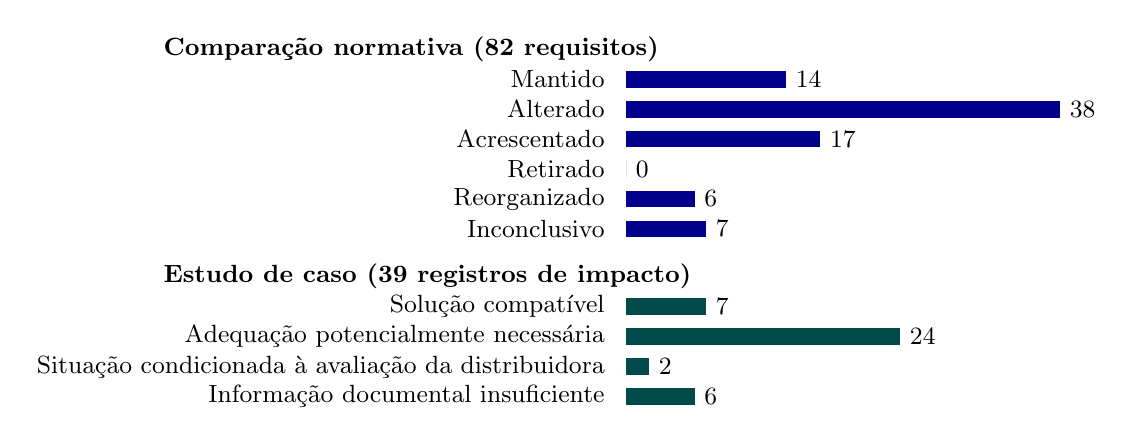
\begin{tikzpicture}[x=1cm, y=0.38cm, font=\small]
  \node[anchor=west, font=\small\bfseries] at (0,0) {Comparação normativa (82 requisitos)};
  \foreach \linha/\categoria/\total in {
    1/Mantido/14,
    2/Alterado/38,
    3/Acrescentado/17,
    4/Retirado/0,
    5/Reorganizado/6,
    6/Inconclusivo/7
  } {
    \node[anchor=east] at (5.85,-\linha) {\categoria};
    \fill[blue!55!black] (6,-\linha-0.28) rectangle ({6+0.145*\total},-\linha+0.28);
    \node[anchor=west] at ({6+0.145*\total},-\linha) {\total};
  }
  \node[anchor=west, font=\small\bfseries] at (0,-7.6) {Estudo de caso (39 registros de impacto)};
  \foreach \linha/\categoria/\total in {
    8.6/Solução compatível/7,
    9.6/Adequação potencialmente necessária/24,
    10.6/Situação condicionada à avaliação da distribuidora/2,
    11.6/Informação documental insuficiente/6
  } {
    \node[anchor=east] at (5.85,-\linha) {\categoria};
    \fill[teal!58!black] (6,-\linha-0.28) rectangle ({6+0.145*\total},-\linha+0.28);
    \node[anchor=west] at ({6+0.145*\total},-\linha) {\total};
  }
\end{tikzpicture}
